\documentclass[journal,12pt,twocolumn]{IEEEtran}
\usepackage{setspace}
\usepackage{gensymb}
\singlespacing
\usepackage[cmex10]{amsmath}

\usepackage{amsthm}
\usepackage{hyperref}
\hypersetup{
    colorlinks=true,
    linkcolor=blue,
    filecolor=magenta,      
    urlcolor=cyan,
}

\urlstyle{same}
\usepackage{mathrsfs}
\usepackage{txfonts}
\usepackage{stfloats}
\usepackage{bm}
\usepackage{cite}
\usepackage{cases}
\usepackage{subfig}

\usepackage{longtable}
\usepackage{multirow}

\usepackage{enumitem}
\usepackage{mathtools}
\usepackage{steinmetz}
\usepackage{tikz}
\usepackage{circuitikz}
\usepackage{verbatim}
\usepackage{tfrupee}
\usepackage[breaklinks=true]{hyperref}
\usepackage{graphicx}
\usepackage{tkz-euclide}
\usetikzlibrary{shapes,backgrounds}
\usepackage{verbatim}
\usetikzlibrary{calc,math}
\usepackage{listings}
    \usepackage{color}                                            %%
    \usepackage{array}                                            %%
    \usepackage{longtable}                                        %%
    \usepackage{calc}                                             %%
    \usepackage{multirow}                                         %%
    \usepackage{hhline}                                           %%
    \usepackage{ifthen}                                           %%
    \usepackage{lscape}     
\usepackage{multicol}
\usepackage{chngcntr}
\usepackage{mdframed}
\DeclareMathOperator*{\Res}{Res}

\renewcommand\thesection{\arabic{section}}
\renewcommand\thesubsection{\thesection.\arabic{subsection}}
\renewcommand\thesubsubsection{\thesubsection.\arabic{subsubsection}}

\renewcommand\thesectiondis{\arabic{section}}
\renewcommand\thesubsectiondis{\thesectiondis.\arabic{subsection}}
\renewcommand\thesubsubsectiondis{\thesubsectiondis.\arabic{subsubsection}}


\hyphenation{op-tical net-works semi-conduc-tor}
\def\inputGnumericTable{}                                 %%

\lstset{
%language=C,
frame=single, 
breaklines=true,
columns=fullflexible
}

\usepackage{chngcntr}
\counterwithin{figure}{section}

\title{AI5002}
\author{TUHIN DUTTA}
\date{January 2021}

\begin{document}
\newtheorem{theorem}{Theorem}[section]
\newtheorem{problem}{Problem}
\newtheorem{proposition}{Proposition}[section]
\newtheorem{lemma}{Lemma}[section]
\newtheorem{corollary}[theorem]{Corollary}
\newtheorem{example}{Example}[section]
\newtheorem{definition}[problem]{Definition}

\newcommand{\BEQA}{\begin{eqnarray}}
\newcommand{\EEQA}{\end{eqnarray}}
\newcommand{\define}{\stackrel{\triangle}{=}}
\bibliographystyle{IEEEtran}
\raggedbottom
\setlength{\parindent}{0pt}
\providecommand{\mbf}{\mathbf}
\providecommand{\pr}[1]{\ensuremath{\Pr\left(#1\right)}}
\providecommand{\qfunc}[1]{\ensuremath{Q\left(#1\right)}}
\providecommand{\sbrak}[1]{\ensuremath{{}\left[#1\right]}}
\providecommand{\lsbrak}[1]{\ensuremath{{}\left[#1\right.}}
\providecommand{\rsbrak}[1]{\ensuremath{{}\left.#1\right]}}
\providecommand{\brak}[1]{\ensuremath{\left(#1\right)}}
\providecommand{\lbrak}[1]{\ensuremath{\left(#1\right.}}
\providecommand{\rbrak}[1]{\ensuremath{\left.#1\right)}}
\providecommand{\cbrak}[1]{\ensuremath{\left\{#1\right\}}}
\providecommand{\lcbrak}[1]{\ensuremath{\left\{#1\right.}}
\providecommand{\rcbrak}[1]{\ensuremath{\left.#1\right\}}}
\theoremstyle{remark}
\newtheorem{rem}{Remark}
\newcommand{\sgn}{\mathop{\mathrm{sgn}}}

\providecommand{\res}[1]{\Res\displaylimits_{#1}} 

%\providecommand{\norm}[1]{\lVert#1\rVert}
\providecommand{\mtx}[1]{\mathbf{#1}}
\providecommand{\fourier}{\overset{\mathcal{F}}{ \rightleftharpoons}}
%\providecommand{\hilbert}{\overset{\mathcal{H}}{ \rightleftharpoons}}
\providecommand{\system}{\overset{\mathcal{H}}{ \longleftrightarrow}}
	%\newcommand{\solution}[2]{\textbf{Solution:}{#1}}
\newcommand{\solution}{\noindent \textbf{Solution: }}
\newcommand{\cosec}{\,\text{cosec}\,}
\providecommand{\dec}[2]{\ensuremath{\overset{#1}{\underset{#2}{\gtrless}}}}
\newcommand{\myvec}[1]{\ensuremath{\begin{pmatrix}#1\end{pmatrix}}}
\newcommand{\mydet}[1]{\ensuremath{\begin{vmatrix}#1\end{vmatrix}}}
\numberwithin{equation}{subsection}
\makeatletter
\@addtoreset{figure}{problem}
\makeatother
\let\StandardTheFigure\thefigure
\let\vec\mathbf
\renewcommand{\thefigure}{\theproblem}
\def\putbox#1#2#3{\makebox[0in][l]{\makebox[#1][l]{}\raisebox{\baselineskip}[0in][0in]{\raisebox{#2}[0in][0in]{#3}}}}
     \def\rightbox#1{\makebox[0in][r]{#1}}
     \def\centbox#1{\makebox[0in]{#1}}
     \def\topbox#1{\raisebox{-\baselineskip}[0in][0in]{#1}}
     \def\midbox#1{\raisebox{-0.5\baselineskip}[0in][0in]{#1}}
\vspace{3cm}
\title{AI5002 - (Compulsory) Assignment}
\author{Tuhin Dutta\\ ai21mtech02002}
\maketitle
\newpage
\bigskip
\renewcommand{\thefigure}{\theenumi}
\renewcommand{\thetable}{\theenumi}
\begin{mdframed}
Download code and LaTeX from below hyperlinks\\
1. \href{https://github.com/Tauhait/AI5002/blob/main/Compulsory-Assignment/Code/Binom\_3\_7.py}{Code/Binom\_3\_7.py}


2. \href{https://github.com/Tauhait/AI5002/tree/main/Compulsory-Assignment/LaTeX}{LaTeX}
\end{mdframed}
\subsection*{\boldsymbol{Problem\ 3.7}}
Let X represent the difference between the number of heads and the number of tails
obtained when a coin is tossed 6 times. What are possible values of X?
Find the pmf/cdf of the difference of two binomial random variables.
\subsection*{\boldsymbol{Solution}}
Let Z represent `Difference between the number of heads and tails when a coin is tossed six times'.\\
\begin{table}[ht]
\centering
\begin{tabular}{c c c}
\hline\hline
\# Heads  & \# Tails  & $Z =\ \#\ Heads - \#\ Tails $\\ [0.5ex]
\hline\hline
0  & 6  & -6 \\
\hline
1  & 5  & -4 \\
\hline
2  & 4  & -2 \\
\hline
3  & 3  & 0 \\
\hline
4  & 2  & 2 \\ 
\hline
5  & 1  & 4 \\
\hline
6  & 0  & 6 \\[1ex]
\hline\hline 
\end{tabular}
\label{table:nonlin}
\caption{\# of Heads, Tails and r.v. Z}
\end{table}
\\Possible values of $Z = \{\ -6,\ -4,\ -2,\ 0,\ 2,\ 4,\ 6\ \}$\\
\begin{align}
    Pr\ (p=\text{`` Head in a single toss ''}) = \dfrac{1}{2}
\end{align}
\begin{align}
    Pr\ (q=\text{`` Tail in a single toss ''}) =  \dfrac{1}{2}
\end{align}
\begin{enumerate}
    \item Note: \pr{p} + \pr{q} = 1\\\\
\end{enumerate}
\text{Let us define two independent binomial r.v.s K and L}.
\begin{multline}
    X = \{ \text{`` Number of heads in six tosses''} \}\\
    X \sim Bin(n=6, p=0.5)
\end{multline}
\begin{multline}
    Y = \{ \text{`` Number of tails in six tosses''} \}\\
    Y \sim Bin(m=6, q=0.5)
\end{multline}
\\
The r.v Z can be represented as -\\
\begin{align}
    Z = X - Y
\end{align}
\\
The binomial pmf is given by - \\
\begin{align}
    \pr{Z = k} = f(k, n, p) = {n \choose k}\ p^k\ (1-p)^{(n-k)}
\end{align}
The probability distribution of the difference of two or more independent random variables is the convolution of their individual distributions.\\
\\
Let k = Y represent all values that Y can take and these implies X = Z + k.
\begin{equation}
    P\ (Z = z)\ &=\ \sum_{k = 0}^{6} P\ (X = z + k)\ .\ P\ (Y = k)
\end{equation}
\begin{equation}
    P\ (Z = z)\ &=\ \sum_{k = 0}^{6} f(z + k,\ n,\ p)\ .\ f(k,\ m,\ q) 
\end{equation}
We define two cases for the positive and negative part of Z, and thus pmf is given as -\\
\begin{align}
\[
    P\ (Z = z)\ &= \left\{\begin{array}{lr}
                    \ \sum_{k = 0}^{n}\ f(z + k,\ n,\ p)\ .\ f(k,\ m,\ q), & z \geq 0\\
                    \\
                    \ \sum_{k = 0}^{m}\ f(k,\ n,\ p)\ .\ f(z + k,\ m,\ q), & z < 0\\
                    \right\}\end{array}
\]\\
\end{align}
\begin{figure}[h!]
    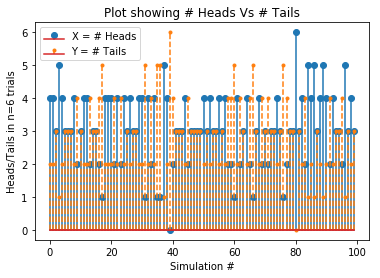
\includegraphics[width=10cm]{Compulsory-Assignment/Code/Figure/binom_3_7_H_vs_T.png}
    \caption*{Fig 1.1: Simulation of X and Y}
\end{figure}
\begin{figure}[h!]
    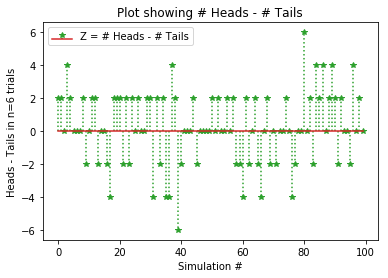
\includegraphics[width=10cm]{Compulsory-Assignment/Code/Figure/binom_3_7_H_-_T.png}
    \caption*{Fig 1.2: Plotting Z = X - Y}
\end{figure}
\end{document}
